\let\negmedspace\undefined
\let\negthickspace\undefined
\documentclass[journal,12pt,twocolumn]{IEEEtran}
\usepackage{cite}
\usepackage{amsmath,amssymb,amsfonts,amsthm}
\usepackage{algorithmic}
\usepackage{graphicx}
\usepackage{textcomp}
\usepackage{xcolor}
\usepackage{txfonts}
\usepackage{listings}
\usepackage{enumitem}
\usepackage{mathtools}
\usepackage{gensymb}
\usepackage{comment}
\usepackage[breaklinks=true]{hyperref}
\usepackage{tkz-euclide} 
\usepackage{listings}
\usepackage{gvv}                                                                                                   
\usepackage{color}                                            
\usepackage{array}                                            
\usepackage{longtable}                                       
\usepackage{calc}                                             
\usepackage{multirow}                                         
\usepackage{hhline}                                           
\usepackage{ifthen}                                           
\usepackage{lscape}

\newtheorem{theorem}{Theorem}[section]
\newtheorem{problem}{Problem}
\newtheorem{proposition}{Proposition}[section]
\newtheorem{lemma}{Lemma}[section]
\newtheorem{corollary}[theorem]{Corollary}
\newtheorem{example}{Example}[section]
\newtheorem{definition}[problem]{Definition}
\newcommand{\BEQA}{\begin{eqnarray}}
\newcommand{\EEQA}{\end{eqnarray}}
\newcommand{\define}{\stackrel{\triangle}{=}}
\theoremstyle{remark}
\newtheorem{rem}{Remark}
\begin{document}

\bibliographystyle{IEEEtran}
\vspace{3cm}

\title{Gaussian 9.3.2}
\author{EE22BTECH11051 Sreekar Cheela}
\maketitle
\newpage
\bigskip
\renewcommand{\thefigure}{\theenumi}
\renewcommand{\thetable}{\theenumi}

\textbf{Question}: There are 5\% defective items in a large bulk of items. What is the probability that a sample of 10 items will include not more than one defective item?\\
\solution 
\begin{table}[h!]
 \begin{center}
    \begin{tabular}{|l|c|r|}
    \hline
    Parameter & Values & Description\\
    \hline
    $n$ & 10 & Number of articles\\
    \hline
    $p$ & 0.05 & Probability of being defective\\
    \hline
    $X$ & $1\leq X \leq 10$
    & X defective elements out of 10\\
    \hline
    $Y$ & $1\leq Y \leq 10$
    & gaussian variable\\
    \hline
    $\mu=np$ & $0.5$ & mean\\
    \hline
    $\sigma=\sqrt{np(1-p)}$ & $0.475$ & standard deviation\\
    \hline
    \end{tabular}
    \end{center}
  \label{table:/9/3/2} 
\end{table}
\begin{enumerate}
    \item Binomial Distribution
\begin{align}
n=10 ; p=\frac{1}{20}
\end{align}
Pmf of $X$ for $0 \leq k \leq 10$ is
\begin{align}
p_X(k)&=\comb{n}{k}p^k(1-p)^{n-k}
\end{align}
Then the probability that in our sample space of 10 items not more than one are defective is given as:
\begin{multline}
p_X(0)+p_X(1)=\comb{10}{0}\left(\frac{1}{20}\right)^0\left(1-\frac{1}{20}\right)^{10}\\
+\comb{10}{1}\left(\frac{1}{20}\right)^1\left(1-\frac{1}{20}\right)^{9}
\end{multline}
Hence we get;
\begin{align}
p_X(0)+p_X(1)=29\left(\frac{19^9}{20^{10}}\right)
            &=0.91386
\end{align}
\item Gaussian Distribution\\
Let Y be our gaussian variable. Now using Central Limit Theroem, we can use the gaussian
distribution function, which is given as:
\begin{align}
p_Y(x)&=\frac{1}{\sqrt{2\pi\sigma^2}}e^{-\frac{(x-\mu)^2}{2\sigma^2}}
\end{align}
Hence the probability of the sample not including more than one defective item is given as;
\begin{align}
    \int\limits_{-\infty}^1 \frac{1}{\sqrt{2\pi\sigma^2}}e^{-\frac{(x-\mu)^2}{2\sigma^2}}dx
    &= 0.765917
\end{align}
\end{enumerate}
\begin{figure}[ht]
    \centering
    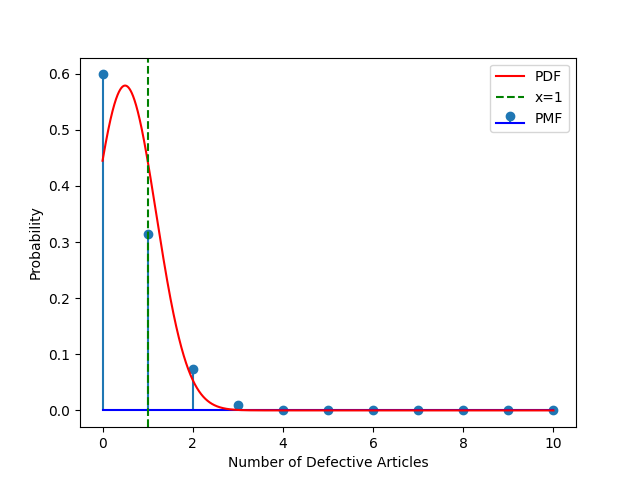
\includegraphics[width=\columnwidth]{./figs/figure1.png}
    \caption{ Binomial-PMF and Gaussian-PDFof $X$}
\end{figure}
\end{document}
